\section{Flag 10 - Guess (hidden folder)}

\paragraph{99dde1d35d1fdd283924d84e6d9f1d820}
\begin{center}
    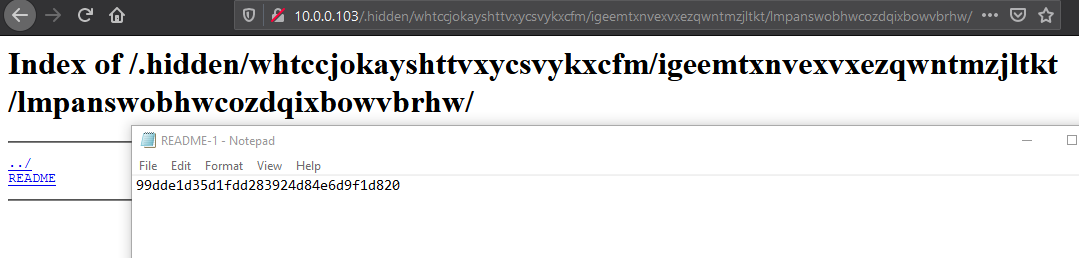
\includegraphics[width=0.5\textwidth]{13.Flag10/10-04.png}\\[0cm] 
\end{center}

\subsection{Vulnerability}

Sensitive data is available to be accessed directly from the URL, hiding it among multiple folders or a complex system does not mean it is invisible or cannot be retrieved. Directory access over the web is not ideal.

\subsection{Location}

'http://<ip-address>:80/.hidden'

\subsection{Method}

The `robots.txt` file lists directories it does not allow to be indexed by 'Web Crawlers'. Access to these directories is not subsequently protected from access.

\subsection{Tools}

\begin{figure}[!htb]
    \centering
    \subfloat[robots.txt]{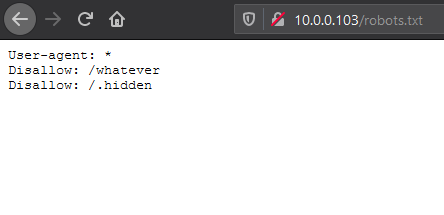
\includegraphics[width=.45\columnwidth]{13.Flag10/10-01.png}\label{fig: 10-01 - wtf}} \quad
    \subfloat[index of /.hidden]{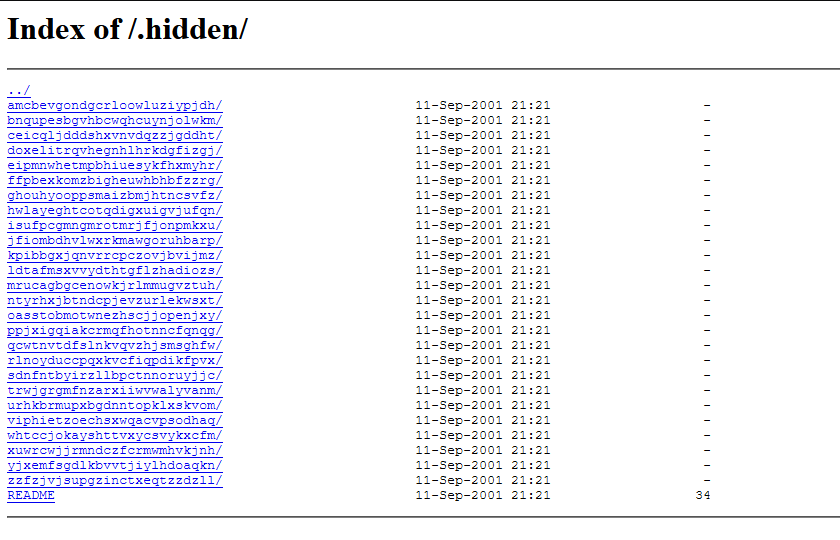
\includegraphics[width=.45\columnwidth]{13.Flag10/10-02.png}\label{fig: 10-02 - wrong}} \\
    \subfloat[Gotcha]{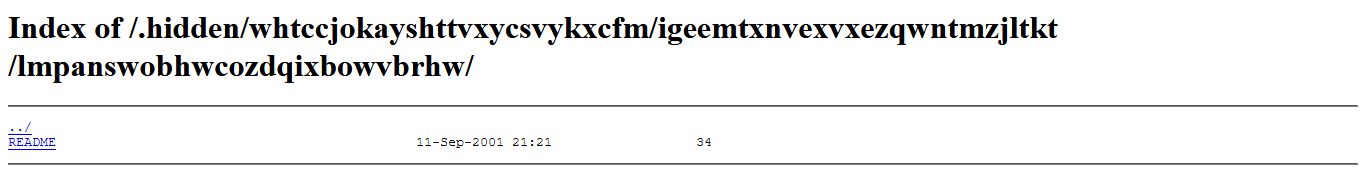
\includegraphics[width=.45\columnwidth]{13.Flag10/10-03.png}\label{fig: 10-03 - wtf}} \quad
    \caption[Flag 10 Method]{Process to Capture the File Hidden Flag} % The text in the square bracket is the caption for the list of figures while the text in the curly brackets is the figure caption
    \label{fig:flag10 method}
\end{figure}

\begin{itemize}
    \item \href{https://www.kali.org/tutorials/kali-on-the-windows-subsystem-for-linux/}{Kali Linux WSL}
    \item \href{https://www.kali.org/docs/wsl/win-kex/}{Kali WSL Win-Kex}
    \item \href{https://daniel.haxx.se/docs/curl-vs-wget.html}{cURL vs Wget}
    \item \href{https://unix.stackexchange.com/questions/47434/what-is-the-difference-between-curl-and-wget}{Unix \& Linux}
    \item \href{https://www.howtogeek.com/281663/how-to-use-wget-the-ultimate-command-line-downloading-tool/}{How To Geek}
    \item \href{https://www.webhostface.com/kb/knowledgebase/examples-using-wget/}{Wget Command Examples}
    \item \href{https://stackoverflow.com/questions/9265172/scrape-an-entire-website}{Stackoverflow - Scrape a website}
    \item \href{https://www.simonholywell.com/post/2015/09/scrape-site-with-wget-and-httrack/}{Scraping websites with wget and httrack}
    \item \href{https://www.linuxjournal.com/content/downloading-entire-web-site-wget}{\textbf{Linux Journal}}    
\end{itemize}

\subsection{Remedy}

\begin{itemize}
    \item Do not store important information on the server.
    \item Disable directories and access to them
\end{itemize}